% xetex compatible variant that support TTF fonts according to company rules
\documentclass[ignorenonframetext, professionalfonts, hyperref={unicode}]{beamer}

\usetheme{Epam}

\usepackage{fontspec}
\setsansfont{SourceSansPro-Regular}
%\setbeamerfont{frametitle}{family=\fontspec{Oswald}}
\setbeamerfont{frametitle}{family=\fontspec{Oswald}}
\setbeamerfont{block title}{family=\fontspec{Oswald}}

%\setmainfont{Times New Roman}
\defaultfontfeatures{Mapping=tex-text}
\defaultfontfeatures{Ligatures=TeX}

%\setsansfont{Arial}
%\setromanfont{Trebuchet MS}

\usepackage{cmap}
\usepackage{graphicx}

\usepackage{textcomp}

\usepackage{beamerthemesplit}

\usepackage{ulem}

\usepackage{verbatim}
\usepackage{import}

\usepackage{listings}
\lstloadlanguages{bash}

\lstset{escapechar=`,
	captionpos=b,
	extendedchars=false,
	language=sh,
%	frame=single,
	tabsize=2, 
	columns=fullflexible, 
%	basicstyle=\scriptsize,
	keywordstyle=\color{blue}, 
	commentstyle=\itshape\color{brown},
%	identifierstyle=\ttfamily, 
	stringstyle=\mdseries\color{green}, 
	showstringspaces=false, 
	numbers=left, 
	numberstyle=\footnotesize, 
	breaklines=true, 
	inputencoding=utf8,
	keepspaces=true,
	morekeywords={u\_short, u\_char, u\_long, in\_addr}
	}

\definecolor{darkgreen}{cmyk}{0.7, 0, 1, 0.5}

\lstdefinelanguage{diff}
{
    morekeywords={+, -},
    sensitive=false,
    morecomment=[l]{//},
    morecomment=[s]{/*}{*/},
    morecomment=[l][\color{darkgreen}]{+},
    morecomment=[l][\color{red}]{-},
    morestring=[b]",
}

\author[Epam]{{\bf Epam}\\Low Level Programming Department}

%\institution[EPAM]{EPAM}
%\logo{\includegraphics[width=1cm]{logo.png}}

\graphicspath{{../../slides/cmdline/clipart/}{../../slides/bash/clipart/}}

\bibliographystyle{unsrt}
\setbeamertemplate{bibliography item}{\insertbiblabel}

\AtBeginSection[]{%
  \begin{frame}<beamer>
    \frametitle{}
    \tableofcontents[
        sectionstyle=show/shaded, hideallsubsections ]
  \end{frame}
  \addtocounter{framenumber}{-1}% If you don't want them to affect the slide number
}

% \regex for regular expressions
\newcommand{\regex}[1]{ %
\expandafter{$\ulcorner{\color{blue}\texttt{#1}}\lrcorner$} %
}



\title{Введение в GNU/Linux}

%%%%%%%%%%%%%%%%%%%%%%%%%%%%%%%%%%%%%%%%%%%%%%%%%
%%%%%%%%%% Begin Document  %%%%%%%%%%%%%%%%%%%%%%
%%%%%%%%%%%%%%%%%%%%%%%%%%%%%%%%%%%%%%%%%%%%%%%%%

\begin{document}

\begin{frame}
	\frametitle{}
	\titlepage
	\vspace{-0.5cm}
	\begin{center}
	%\frontpagelogo
	\end{center}
\end{frame}


\begin{frame}
	\tableofcontents
	[hideallsubsections]
\end{frame}

%%%%%%%%%%%%%%%%%%%%%%%%%%%%%%%%%%%%%%%%%   
%%%%%%%%%% Content starts here %%%%%%%%%%
%%%%%%%%%%%%%%%%%%%%%%%%%%%%%%%%%%%%%%%%%

\section{Работа с файлами в файловой системе.}
\mode<all>{\begin{frame}[fragile]{Путь к файлу.}
      \begin{itemize}
        \item Имя файла
                \begin{itemize}
                    \item чувствительно к регистру
                    \item / разделяет директории
                    \item - \textbackslash <Space> специальные символы 
                    \item . скрытый файл
                \end{itemize}
        \item \alert{Полное имя файла} (absolute pathname) начинается с /
        \item \alert{Относительное имя файла} (relative pathname) начинается с
        любого другого символа. Поиск файла производится относительно
        \alert{текущей директории} (current working directory).
      \end{itemize}

      \begin{block}{Примеры}
        ./ - текущая директория

        ../ - предыдущая директория

        ../../usr/bin/ls

        /usr/bin/ls
      \end{block}
\end{frame}

\begin{frame}[fragile]{Навигация по файловой системе}
      \begin{itemize}
		  \item {\tt pwd} -- имя текущей директории (help pwd)
		  \item {\tt ls} -- список файлов в директории. По умолчанию в текущей (man ls)
		  \item {\tt cd} -- смена текущей директории (help cd)
      \end{itemize}
      \begin{block}{Упражнение. Заходим в /usr/bin/ и просматриваем список доступных команд.}
	\begin{lstlisting}
	pwd
	cd /usr/bin/
	pwd
	ls
	cd -	
	pwd
	\end{lstlisting}
      \end{block}
\end{frame}

\begin{frame}[fragile]{Просмотр типов файлов}
      \begin{block}{Упражнение. Символьное обозначение типа файла.}
Первая буква вывода команды ls -l обозначает тип файла. 
Tip. Команды file позволяет определить тип файла. Ключ -d для работы с
директорией. 

/dev/zero

/dev/sda 

.. 

/bin/sh 

/dev/log

/dev/stdout
      \end{block}
\end{frame}

\begin{frame}[fragile]{Команды для работы с файлами}
	\begin{itemize}
		\begin{columns}
		\column{0.2\textwidth}
			\item touch
			\item ln
			\item mkdir
			\item mknod
			\item mkfifo

		\column{0.2\textwidth}
			\item cp
			\item mv
			\item rm
			\item rmdir
			\item file
			\item install

		\column{0.4\textwidth}
			\begin{block}{Упражнение}
				\begin{enumerate}
					\item Создать иерархию директорий
						\begin{lstlisting}
dir1/dir1.1/dir1.1.1
dir1/dir1.2/dir1.2.1
dir1/dir1.2/dir1.2.2
						\end{lstlisting}
					\item Внутри каждой создать файл
					\item Удалить все созданное
				\end{enumerate}
			\end{block}
			
		\end{columns}
	\end{itemize}
\end{frame}
}
\section{Файловая система.}
\mode<all>{
\begin{frame}{Детали реализации}
  \begin{itemize}
    \item \alert{VFS - virtual file system} - файлы и каталоги отображаются в единое дерево, независимо от их физического расположения.
  \end{itemize}
  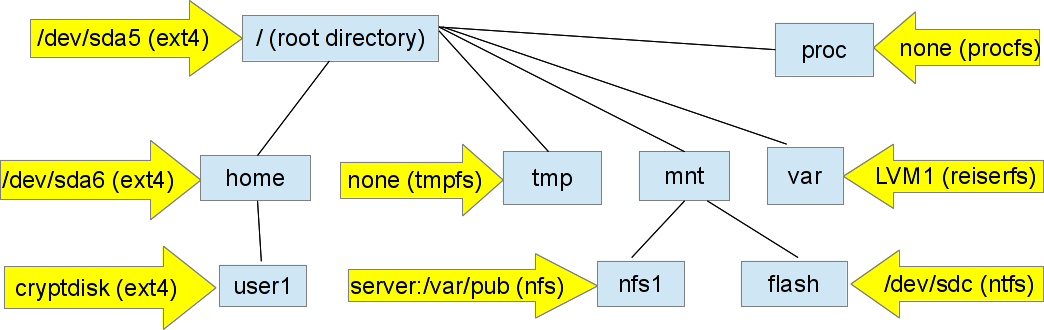
\includegraphics[height=3.5cm]{vfs-and-devices}
\end{frame}

\begin{frame}{Монтирование}
  \begin{itemize}
    \item \alert{Монтирование} - процесс отображения содержимого устройства в указанную папку файловой системы.
    \item Команды:
      \begin{itemize}
        \item монтировать - ( \alert{mount} ) 
        \item размонтировать ( \alert{umount} )
      \end{itemize}
    \item \alert{mount} без параметров - вывести список уже подключенных файловых систем
  \end{itemize}
      \begin{block}{Упражнение. Дерево монтирования.}
     Получить вывод смонтированных блочных устройств в виде дерева с помощью команды: \alert{findmnt}
      \end{block}
  
\end{frame}

}
\section{Создание файловой системы.}
\mode<all>{\begin{frame}{Disk management tools}
	\begin{columns}
		\column{0.25\textwidth}
		\begin{itemize}
			\item {\tt fdisk}
			\item {\tt parted}
			\item {\tt kpartx}
		\end{itemize}
		\column{0.25\textwidth}
		\begin{itemize}
			\item {\tt dd}
			\item {\tt losetup}
		\end{itemize}
		\column{0.25\textwidth}
		\begin{itemize}
			\item {\tt mkfs}
			\item {\tt fsck}
		\end{itemize}
		\column{0.25\textwidth}
		\begin{itemize}
			\item {\tt mount}
			\item {\tt umount}
			\item {\tt df}
		\end{itemize}
	\end{columns}
\end{frame}
}
\section{Поиск файлов}
\mode<all>{\begin{frame}[fragile]{Файловая система. Данные и метаданные.}
    \begin{columns}
        \column{0.6\textwidth}
  \begin{block}{Упражнение. Выполнить команды. Расскажите что получили.}
    cat /etc/passwd
    \break
    stat /etc/passwd
  \end{block} 
        \column{0.3\textwidth}
        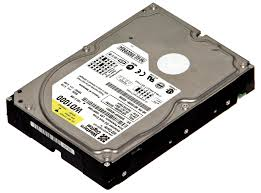
\includegraphics[height=3cm]{hw_hdd.jpg} 
    \end{columns}
\pause
Матаданные - информация о файле.
\begin{itemize}
 \item Размер файла
 \item Владелец и права доступа 
 \item Время доступа, изменения
\end{itemize}
\end{frame}
}
\mode<all>{\begin{frame}[fragile]{Поиск файлов командой find}
    \alert{find} ищет файлы в заданной директории и производит над ним заданную операцию.
	\begin{block}{Часто используемые параметры поиска}
		\begin{itemize}
			\item {\tt -name}, {\tt -iname} -- имя файлового объекта, включая метасимволы 
			\item {\tt -type} -- тип файлового объекта
			\item {\tt -size} -- размер [cwbkMG]
			\item {\tt -perm} -- права доступа
			\item {\tt -user} -- владелец
			\item {\tt ...} -- другие опции man find 
		\end{itemize}
	\end{block}
\end{frame}

\begin{frame}[fragile]{Файлы найдены}
	\begin{block}{Действия над результом поиска}
		\begin{itemize}
			\item {\tt -print} -- вывод на stdout (по умолчанию)
			\item {\tt -printf} -- форматированный вывод
			\item {\tt -exec} -- выполнить команду
			\item {\tt -ls} -- замена -exec ls -l \{\} ;
			\item {\tt -delete} -- удалить файл
		\end{itemize}
	\end{block}
\end{frame}

\begin{frame}[fragile]{Примеры использования команды find}
            В текущей директории найти все файлы *.o и вывести на экран 
            \begin{verbatim} find . -name '*.o' -print \end{verbatim}
            \begin{verbatim} find -name '*.o' \end{verbatim}
            Поск по типу и владельцу файла.
            \begin{verbatim} find -type d -user altlinux \end{verbatim}
            Составная команда, множество условий
            \begin{verbatim} find /root \( -name '*.pyc' -o -name '*.py' \) \
-type f -user root -size +300k -size -1024k \
-exec ls -l \{\} \; \end{verbatim}
 Дополнительно: позволяет преодолеть лимит на кол-во аргументов в командной строке. 
 \textquotedblleft Arguments too long.\textquotedblright 
\end{frame}

\begin{frame}[fragile]{xargs}
			Утилита для создания и запуска команд из стандартного потока ввода:
		\begin{verbatim}
xargs [options] command [command options]
                \end{verbatim}
		\begin{itemize}
			\item {\tt -d} -- разделитель
			\item {\tt -0} -- null-terminated строки
			\item {\tt -I text} -- подстановка
			\item {\tt -n N} -- максимальное количество аргументов
			\item {\tt -P N} -- максимальное количество процессов
		\end{itemize}

%Для работы с разделителями в имени файла: пробелы, tab, символ новой строки. 
Использовать -print0 в команде find для замены на ASCII NUL в имени файла.
\end{frame}

\begin{frame}[fragile]{xargs}
	\begin{block}{Примеры}
		\begin{verbatim}
file /bin/*  | grep shell | cut -f 1 -d ':' | xargs wc -l 
# calculate number of strings in all shell scripts
                \end{verbatim}
		\begin{verbatim}
find /etc -type f -size -100k | \
 xargs tar -czf /tmp/archive-100k.tar.gz
                \end{verbatim}
		\begin{verbatim}
find /etc -type f | xargs -I {} echo "Найден {} файл"
                \end{verbatim}

		\begin{verbatim}
find . -type f -name "*.mp3" -print0 | \
 xargs -0 -n 1 -P 0 -I mp3 avconv -i mp3 mp3.ogg
                \end{verbatim}
	
	\end{block}
\end{frame}
}
%\mode<all>{\begin{frame}[fragile]{xargs}
			Утилита для создания и запуска команд из стандартного потока ввода:
		\begin{verbatim}
xargs [options] command [command options]
                \end{verbatim}
		\begin{itemize}
			\item {\tt -d} -- разделитель
			\item {\tt -0} -- null-terminated строки
			\item {\tt -I text} -- подстановка
			\item {\tt -n N} -- максимальное количество аргументов
			\item {\tt -P N} -- максимальное количество процессов
		\end{itemize}

%Для работы с разделителями в имени файла: пробелы, tab, символ новой строки. 
Использовать -print0 в команде find для замены на ASCII NUL в имени файла.
\end{frame}

\begin{frame}[fragile]{xargs}
	\begin{block}{Примеры}
		\begin{verbatim}
file /bin/*  | grep shell | cut -f 1 -d ':' | xargs wc -l 
# calculate number of strings in all shell scripts
                \end{verbatim}
		\begin{verbatim}
find /etc -type f -size -100k | \
 xargs tar -czf /tmp/archive-100k.tar.gz
                \end{verbatim}
		\begin{verbatim}
find /etc -type f | xargs -I {} echo "Найден {} файл"
                \end{verbatim}

		\begin{verbatim}
find . -type f -name "*.mp3" -print0 | \
 xargs -0 -n 1 -P 0 -I mp3 avconv -i mp3 mp3.ogg
                \end{verbatim}
	
	\end{block}
\end{frame}
} % to video
\end{document}
\bye
